\documentclass[a4paper,11pt]{article}
\usepackage{fullpage}
\usepackage[latin1]{inputenc}
\usepackage[T1]{fontenc}
\usepackage[normalem]{ulem}
\usepackage[english]{babel}
\usepackage{listings,babel}
\lstset{breaklines=true,basicstyle=\ttfamily}
\usepackage{graphicx}
\usepackage{moreverb}
\usepackage{float}
\usepackage{url}
\usepackage{tabularx}

\title{Configuration and Status Register (CSR) bus specifications}
\author{S\'ebastien Bourdeauducq}
\date{December 2009}
\begin{document}
\setlength{\parindent}{0pt}
\setlength{\parskip}{5pt}
\maketitle{}
\section{Introduction}
The CSR bus is designed to provide a lightweight interface to the configuration and status registers (CSRs) of peripherals.

It is built on the following principles:
\begin{itemize}
\item Synchronism. The bus is meant to be used in FPGA-based devices, whose architectures are designed for synchronous (clock-driven) systems.
\item Low signal count. There is no need for signals that take care of variable latency and qualification of accesses; since CSRs are often actual registers (D flip-flops) that can always be read or written at anytime within one cycle. There is no need for a large address bus; a fairly complicated SoC only contains about a thousand CSRs.
\item Low performance. Performance and associated complications are not needed for CSRs.
\item High routability. The CSR bus must often span several devices in the chip that can be physically separated by a large distance, resulting in large routing and load delays. To avoid creating critical paths on the bus, the protocol must ease implementations with little combinatorial logic at endpoints.
\end{itemize}

\section{Specifications}
\subsection{Signals}
A CSR interface is made up of the following signals:

\begin{tabularx}{\textwidth}{|l|l|l|X|}
\hline
\bf{Signal} & \bf{Width} & \bf{Direction} & \bf{Description} \\
\hline
a & 14 & Master to slave & Address signals. The upper 4 bits are used to select a slave, and the lower 10 to select a register within that slave. \\
\hline
we & 1 & Master to slave & Write enable signal. \\
\hline
dw & 32 & Master to slave & Write data. \\
\hline
dr & 32 & Slave to master & Read data. \\
\hline
\end{tabularx}\\

The operation is the same as that of a synchronous SRAM; except that it only responds when the upper 4 address bits are set to a particular value. The read and write cycles are detailed below.

\subsection{Read cycle}
The master initiates a read cycle by positioning the address lines in accordance with the device and register it wants to read. The write enable signal is set to 0.

The upper 4 address bits are used to select a slave. A single CSR bus can span up to 16 slaves. The lower 10 bits are used to select a register within a slave. Each slave can have up to 1024 registers.

The slave responds at the next clock cycle by positioning the contents of the requested register on the read data lines. The operation is pipelined, ie. while the slave responds, the master can position the address lines to read a register again at the next cycle.

If the slave is not selected (the upper 4 bits are not set to its address), it must assert 0 on all data read lines.

Here is an example timing diagram of read cycles to a slave responding to address 6:

\begin{tabular}{|l|c|c|c|c|c|c|c|}
\hline
a & 5.2 & 3.1 & 6.1 & 3.1 & 6.42 & 6.12 & 12.321 \\
\hline
we & 0 & 0 & 0 & 0 & 0 & 0 & 0 \\
\hline
dw & X & X & X & X & X & X & X \\
\hline
dr & 0 & 0 & 0 & Reg 1 & 0 & Reg 42 & Reg 12 \\
\hline
\end{tabular}

X = don't care

a.b = bit vector made by concatening the binary representations of a (4-bit) and b (10-bit)

\subsection{Write cycle}
The master initiates a write cycle by presenting valid data on \verb!dw!, asserting \verb!we!, and positioning the address lines in accordance with the slave and register it wants to write to.

As for read cycles, the upper 4 bits are used to select a slave, and the lower 10 bits are used to select a register within that slave.

If the slave is not selected, it ignores the write cycle. If it is selected, it writes its register at the next cycle.

After a write cycle (\verb!we=1!), the data read lines are invalid, no matter whether a slave was selected or not.

It is possible to issue two or more consecutive write cycles.

Here is an example timing diagram of write and read cycles to a slave responding to address 6:

\begin{tabular}{|l|c|c|c|c|c|c|c|}
\hline
a & 5.2 & 3.1 & 6.1 & 3.1 & 6.42 & 6.12 & 12.321 \\
\hline
we & 1 & 0 & 1 & 0 & 1 & 0 & 0 \\
\hline
dw & 32 & X & 12 & X & 143 & X & X \\
\hline
dr & 0 & X & 0 & X & 0 & X & Reg 12 \\
\hline
Writes & -- & -- & -- & $12\to1$ & -- & $143\to42$ & -- \\
\hline
\end{tabular}

\section{Bus topology}

\begin{figure}[H]
\centering
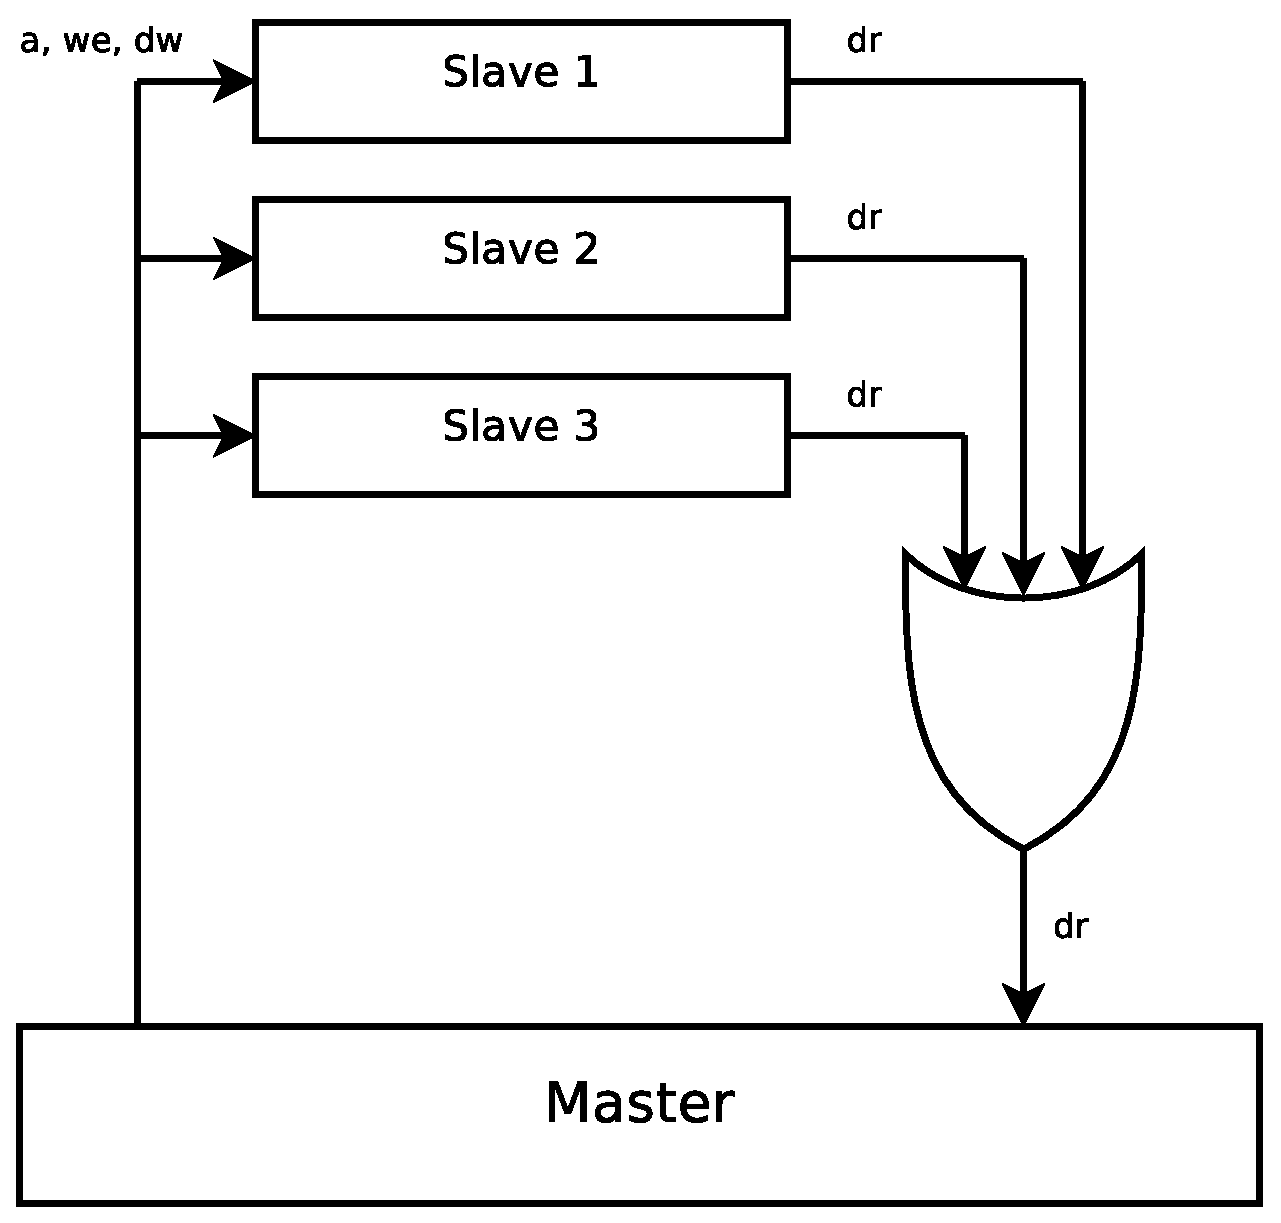
\includegraphics[height=80mm]{csr_topology.eps}
\caption{Example CSR bus topology}
\end{figure}

To combine several CSR buses so that many slaves can be accessed by a single master, the following connections should be made:
\begin{itemize}
\item connect all \verb!a!, \verb!we! and \verb!dw! signals together (master to slave path).
\item perform a bitwise OR on all \verb!dr! outputs of the slaves, and connect the output of the OR to the \verb!dr! input of the master (slave to master path).
\end{itemize}
With these connections, the master can access multiple slaves as if it it was connected to only one.
This topology is similar to the ``distributed OR'' topology of the DCR bus in the IBM CoreConnect architecture, and has the same advantages.

\section*{Copyright notice}
Copyright \copyright 2007-2009 S\'ebastien Bourdeauducq. \\
Permission is granted to copy, distribute and/or modify this document under the terms of the GNU Free Documentation License, Version 1.3; with no Invariant Sections, no Front-Cover Texts, and no Back-Cover Texts. A copy of the license is included in the LICENSE.FDL file at the root of the Milkymist source distribution.

\end{document}
